\documentclass[11pt,a4paper]{article}
\usepackage[utf8]{inputenc}
\usepackage[spanish,es-nodecimaldot]{babel}
\usepackage{geometry}
\usepackage{booktabs}
\usepackage{graphicx}
\usepackage{float}
\usepackage{amsmath,amssymb}
\usepackage{hyperref}
\usepackage{xcolor}
\usepackage{microtype}
\usepackage{enumitem}

\geometry{top=2cm,bottom=2cm,left=2.2cm,right=2.2cm}
\setlength{\parskip}{5pt}
\setlength{\parindent}{0pt}

\definecolor{navyblue}{RGB}{15,37,55}
\definecolor{darkgold}{RGB}{184,134,11}

\hypersetup{
    colorlinks=true,
    linkcolor=navyblue,
    citecolor=navyblue,
    urlcolor=navyblue
}

\graphicspath{{../04_graficos/}{04_graficos/}{./}}

\title{\vspace{-1.2cm}\Large\bfseries\color{navyblue} INFORME EJECUTIVO: ¿25\% ANUAL SIN CAÍDAS?\\
\large\textit{El Veredicto del Modelo CAPM sobre 10 Expedientes de Inversión}}

\author{\textbf{Julián Duarte} \\
Ciencia de Datos | Valoración de Activos (DEFI 2) -- Universidad Externado de Colombia}
\date{Agosto de 2026}

\begin{document}
\maketitle

\begin{abstract}
\noindent Este informe evalúa el caso planteado por la familia de Doña Victoria: la búsqueda de una rentabilidad del 25\% anual sin asumir caídas de capital. Desde la perspectiva de la ciencia de datos aplicada a la valoración de activos, se utiliza el modelo CAPM como filtro cuantitativo sobre 10 expedientes (un criptoactivo: Solana, y nueve acciones de bajo precio en Tecnología, Biotecnología y Energía) para analizar si el mercado realmente recompensa el riesgo asumido. La evidencia empírica con 499 días de datos demuestra que el objetivo es un espejismo financiero: las opciones de alto retorno sufren caídas acumuladas destructivas de hasta el -93.9\% y sufren de severa iliquidez. Se presenta una propuesta clara y explicativa estructurada para tres mandatos de inversión.
\end{abstract}

\hrule
\vspace{0.2cm}

\section{El Dilema de Doña Victoria: ¿Es posible ganar 25\% sin riesgo?}

Cuando una familia busca proteger y multiplicar su patrimonio, la promesa de altos rendimientos resulta sumamente atractiva. Doña Victoria plantea una pregunta fundamental: \textit{¿podemos lograr un 25\% anual sin arriesgar el capital a caídas severas?}

Como estudiantes de Ciencia de Datos aplicados a la valoración de activos, nuestro deber no es validar ilusiones financieras, sino aplicar herramientas cuantitativas para medir el costo real del riesgo. Para este estudio, pusimos bajo la lupa \textbf{10 expedientes de inversión}:
\begin{enumerate}[leftmargin=*]
    \item \textbf{Criptoactivo:} Solana (\texttt{SOL}) comparado contra el índice general cripto \textit{Nasdaq Crypto Index} (\texttt{NCI}).
    \item \textbf{Sector Tecnología:} Kopin (\texttt{KOPN}), MicroVision (\texttt{MVIS}) y AEye (\texttt{LIDR}) frente al ETF sectorial de tecnología (\texttt{XLK}).
    \item \textbf{Sector Biotecnología:} Geron (\texttt{GERN}), CytomX (\texttt{CTMX}) y Ocugen (\texttt{OCGN}) frente al ETF de biotecnología (\texttt{XBI}).
    \item \textbf{Sector Energía:} Borr Drilling (\texttt{BORR}), KLX Energy (\texttt{KLXE}) y TETRA Technologies (\texttt{TTI}) frente al ETF de energía (\texttt{XLE}).
\end{enumerate}

\section{Los Datos y la Herramienta de Medición}

Analizamos un periodo de dos años (agosto de 2024 a agosto de 2026) con 499 días de negociación. Se utilizaron precios ajustados y volúmenes de Yahoo Finance, el registro oficial del índice \texttt{NCI} y la tasa de interés de los Títulos del Tesoro a 3 meses (\texttt{DGS3MO}) como referencia de activo libre de riesgo.

Para entender los resultados sin caer en tecnicismos innecesarios, el modelo CAPM utiliza dos indicadores clave:
\begin{itemize}[leftmargin=*]
    \item \textbf{La Beta ($\beta$):} Mide qué tan sensible es un activo frente a su mercado. Una beta mayor a 1.0 significa que el activo se mueve como un "amplificador" (sube más cuando el mercado sube, pero cae mucho más fuerte cuando el mercado cae).
    \item \textbf{El Alfa de Jensen ($\alpha$):} Mide la recompensa neta. Muestra si el activo generó un retorno verdadero por encima de lo que exigía el riesgo de su beta.
\end{itemize}

\section{El Veredicto Econométrico: Quién paga el riesgo y quién lo destruye}

La Tabla \ref{tab:capm} muestra los resultados de las estimaciones utilizando errores robustos para corregir volatilidad e hiperactividad de precios.

\begin{table}[H]
\centering
\caption{Resultados del Modelo CAPM para los 10 Expedientes}
\label{tab:capm}
\resizebox{\linewidth}{!}{%
\begin{tabular}{lcccccccc}\toprule
\textbf{Activo} & \textbf{Mercado Ref.} & $\mathbf{\hat{\alpha}_{\text{anual}}}$ & $\mathbf{\hat{\beta}}$ & \textbf{Intervalo Beta} & $\mathbf{R^2}$ & \textbf{Ret. Realizado} & \textbf{Ret. Exigido CAPM} & \textbf{Veredicto Neto} \\\midrule
\texttt{SOL}  & NCI & -28.86\% & 1.25 & [1.16, 1.34] & 0.66 & 4.62\%  & 33.48\% & \color{red}Destruye valor (-28.8pp) \\
\texttt{KOPN} & XLK & +80.66\% & 1.82 & [1.57, 2.07] & 0.23 & 129.96\% & 49.31\% & \color{green!60!black}Paga Alfa (+80.6pp) \\
\texttt{MVIS} & XLK & -82.91\% & 1.16 & [0.84, 1.47] & 0.09 & -50.14\% & 32.76\% & \color{red}Trampa de riesgo (-82.9pp) \\
\texttt{LIDR} & XLK & +60.13\% & 1.27 & [0.96, 1.58] & 0.04 & 95.74\%  & 35.61\% & \color{green!60!black}Paga Alfa (+60.1pp) \\
\texttt{GERN} & XBI & -64.14\% & 1.12 & [0.98, 1.27] & 0.22 & -32.87\% & 31.27\% & \color{red}Insuficiente (-64.1pp) \\
\texttt{CTMX} & XBI & +72.75\% & 1.52 & [0.90, 2.13] & 0.11 & 113.54\% & 40.79\% & \color{green!60!black}Paga Alfa (+72.7pp) \\
\texttt{OCGN} & XBI & -2.30\%  & 1.15 & [0.96, 1.34] & 0.17 & 29.60\%  & 31.90\% & \color{red}Neutral / Brecha negativa \\
\texttt{BORR} & XLE & -29.54\% & 1.36 & [1.11, 1.60] & 0.27 & -0.62\%  & 28.91\% & \color{red}Destruye valor (-29.5pp) \\
\texttt{KLXE} & XLE & -67.77\% & 1.94 & [1.59, 2.29] & 0.20 & -28.20\% & 39.56\% & \color{red}Sensibilidad destructiva \\
\texttt{TTI}  & XLE & +29.83\% & 1.14 & [0.87, 1.40] & 0.18 & 54.68\%  & 24.85\% & \color{green!60!black}Paga Alfa (+29.8pp) \\\bottomrule
\end{tabular}%
}
\end{table}

\begin{figure}[H]
\centering
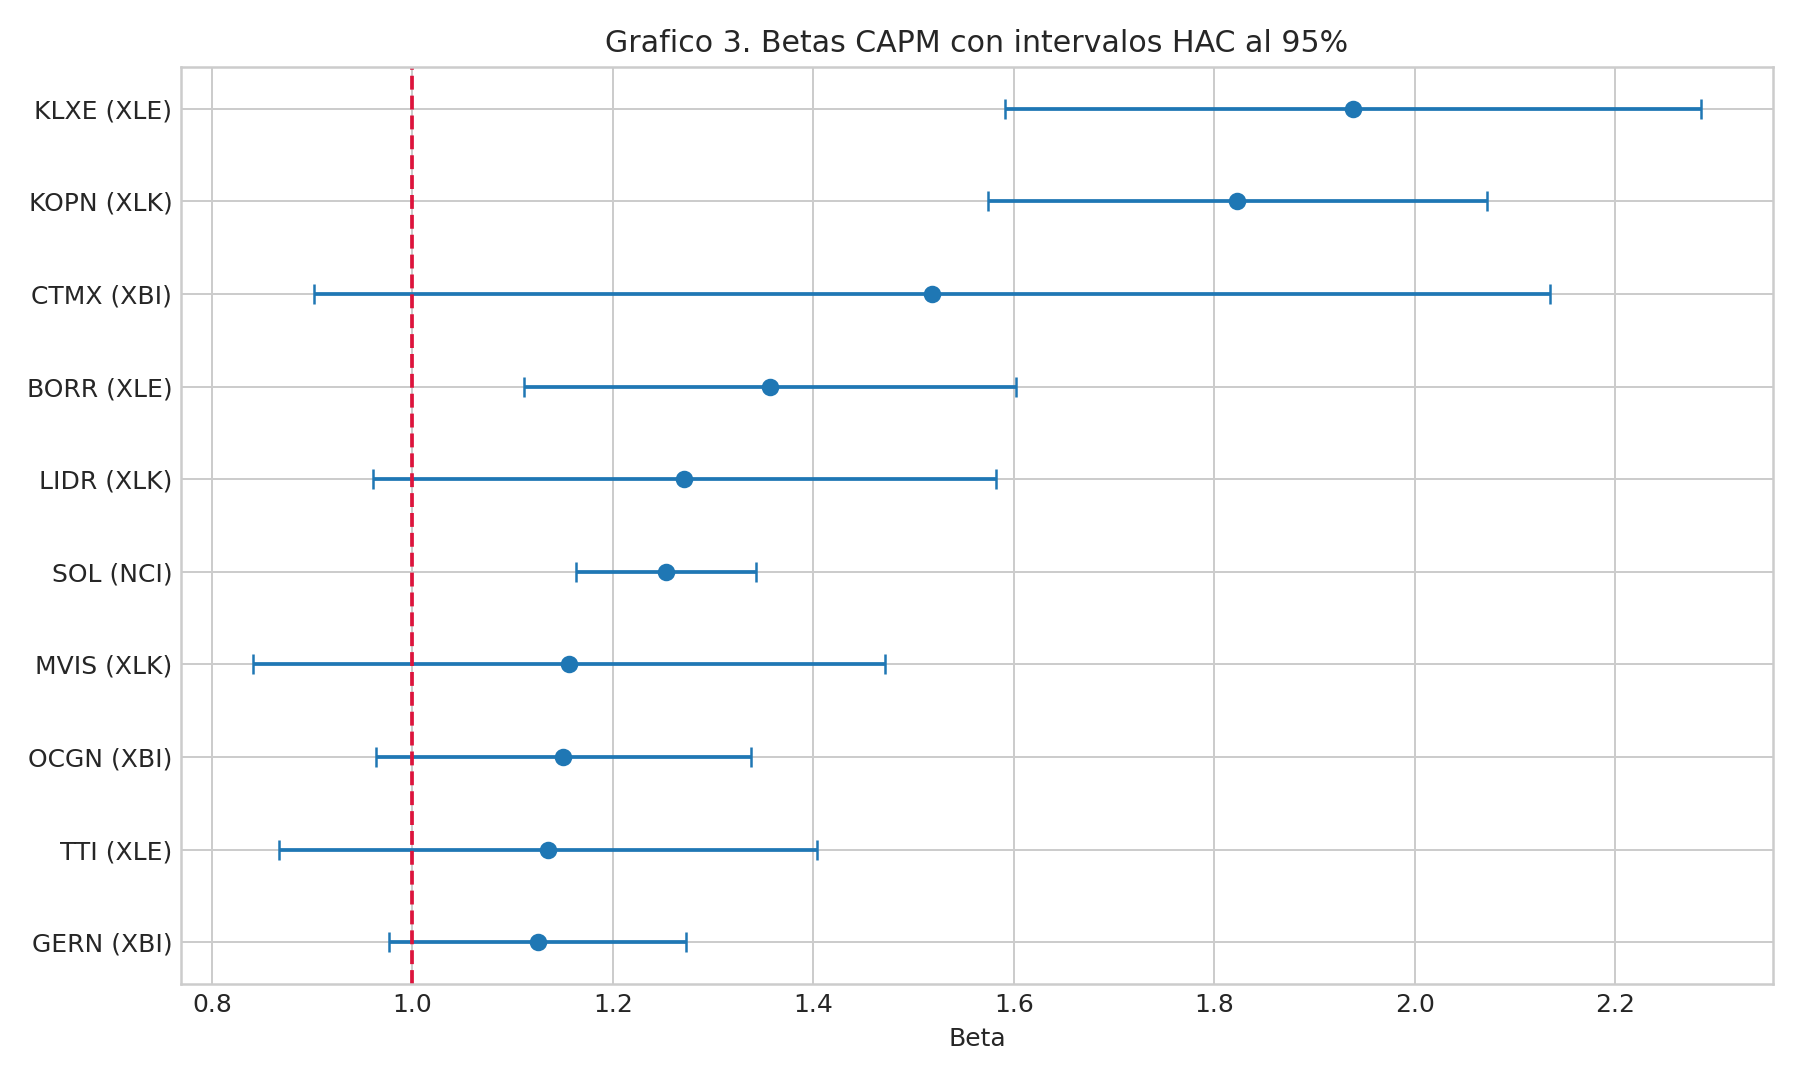
\includegraphics[width=0.82\linewidth]{grafico_3_forest_plot_betas.png}
\caption{Sensibilidad (Beta) de cada activo. Cada beta debe evaluarse únicamente frente a su mercado de referencia propio; no se pueden comparar betas de cripto directamente con betas de energía.}
\label{fig:forest}
\end{figure}

El resultado es contundente: \textbf{solo 4 de los 10 activos (\texttt{KOPN}, \texttt{LIDR}, \texttt{CTMX} y \texttt{TTI}) lograron generar retornos por encima del riesgo de su beta}. Los otros 6 activos destruyeron patrimonio en comparación con lo que el mercado exigía.

\section{La Caída que el Promedio Oculta: Drawdowns y Liquidez}

Un inversionista no vive del promedio aritmético; vive la trayectoria del día a día. Aunque un activo prometa subir a largo plazo, una caída extrema puede quebrantar la estabilidad de cualquier familia.

\begin{table}[H]
\centering
\caption{Métricas de Riesgo Real: Caídas Máximas e Iliquidez}
\label{tab:riesgo}
\resizebox{\linewidth}{!}{%
\begin{tabular}{lcccccp{5cm}}\toprule
\textbf{Activo} & \textbf{Volatilidad Anual} & \textbf{Max Drawdown (MDD)} & \textbf{Peor Pérdida Día (CVaR)} & \textbf{\% Días Retorno 0} & \textbf{Diagnóstico de Liquidez} \\\midrule
\texttt{SOL}  & 88.00\%  & -75.45\% & -9.99\%  & 0.0\%  & Alta liquidez cripto, caídas muy profundas \\
\texttt{KOPN} & 103.28\% & -63.55\% & -12.35\% & 3.6\%  & Genera alfa pero con fuerte volatilidad \\
\texttt{MVIS} & 104.55\% & -93.92\% & -15.14\% & 11.0\% & Destrucción de capital extrema y trampas \\
\texttt{LIDR} & 165.91\% & -82.98\% & -14.09\% & 3.8\%  & Alfa positivo pero riesgo severo de salida \\
\texttt{GERN} & 66.55\%  & -77.47\% & -8.69\%  & 8.0\%  & Sensible a noticias biotecnológicas \\
\texttt{CTMX} & 128.34\% & -67.02\% & -11.49\% & 3.2\%  & Alfa biotecnológico con riesgo elevado \\
\texttt{OCGN} & 77.83\%  & -61.20\% & -9.18\%  & 5.8\%  & No compensa el riesgo tomado \\
\texttt{BORR} & 61.72\%  & -74.78\% & -8.00\%  & 4.4\%  & Alta sensibilidad al petróleo sin premio \\
\texttt{KLXE} & 100.92\% & -79.89\% & -12.95\% & 3.4\%  & Máxima beta ($\beta=1.94$) con fuerte iliquidez \\
\texttt{TTI}  & 62.21\%  & -57.23\% & -8.40\%  & 2.0\%  & Menor caída del grupo de penny stocks \\\bottomrule
\end{tabular}%
}
\end{table}

\begin{figure}[H]
\centering
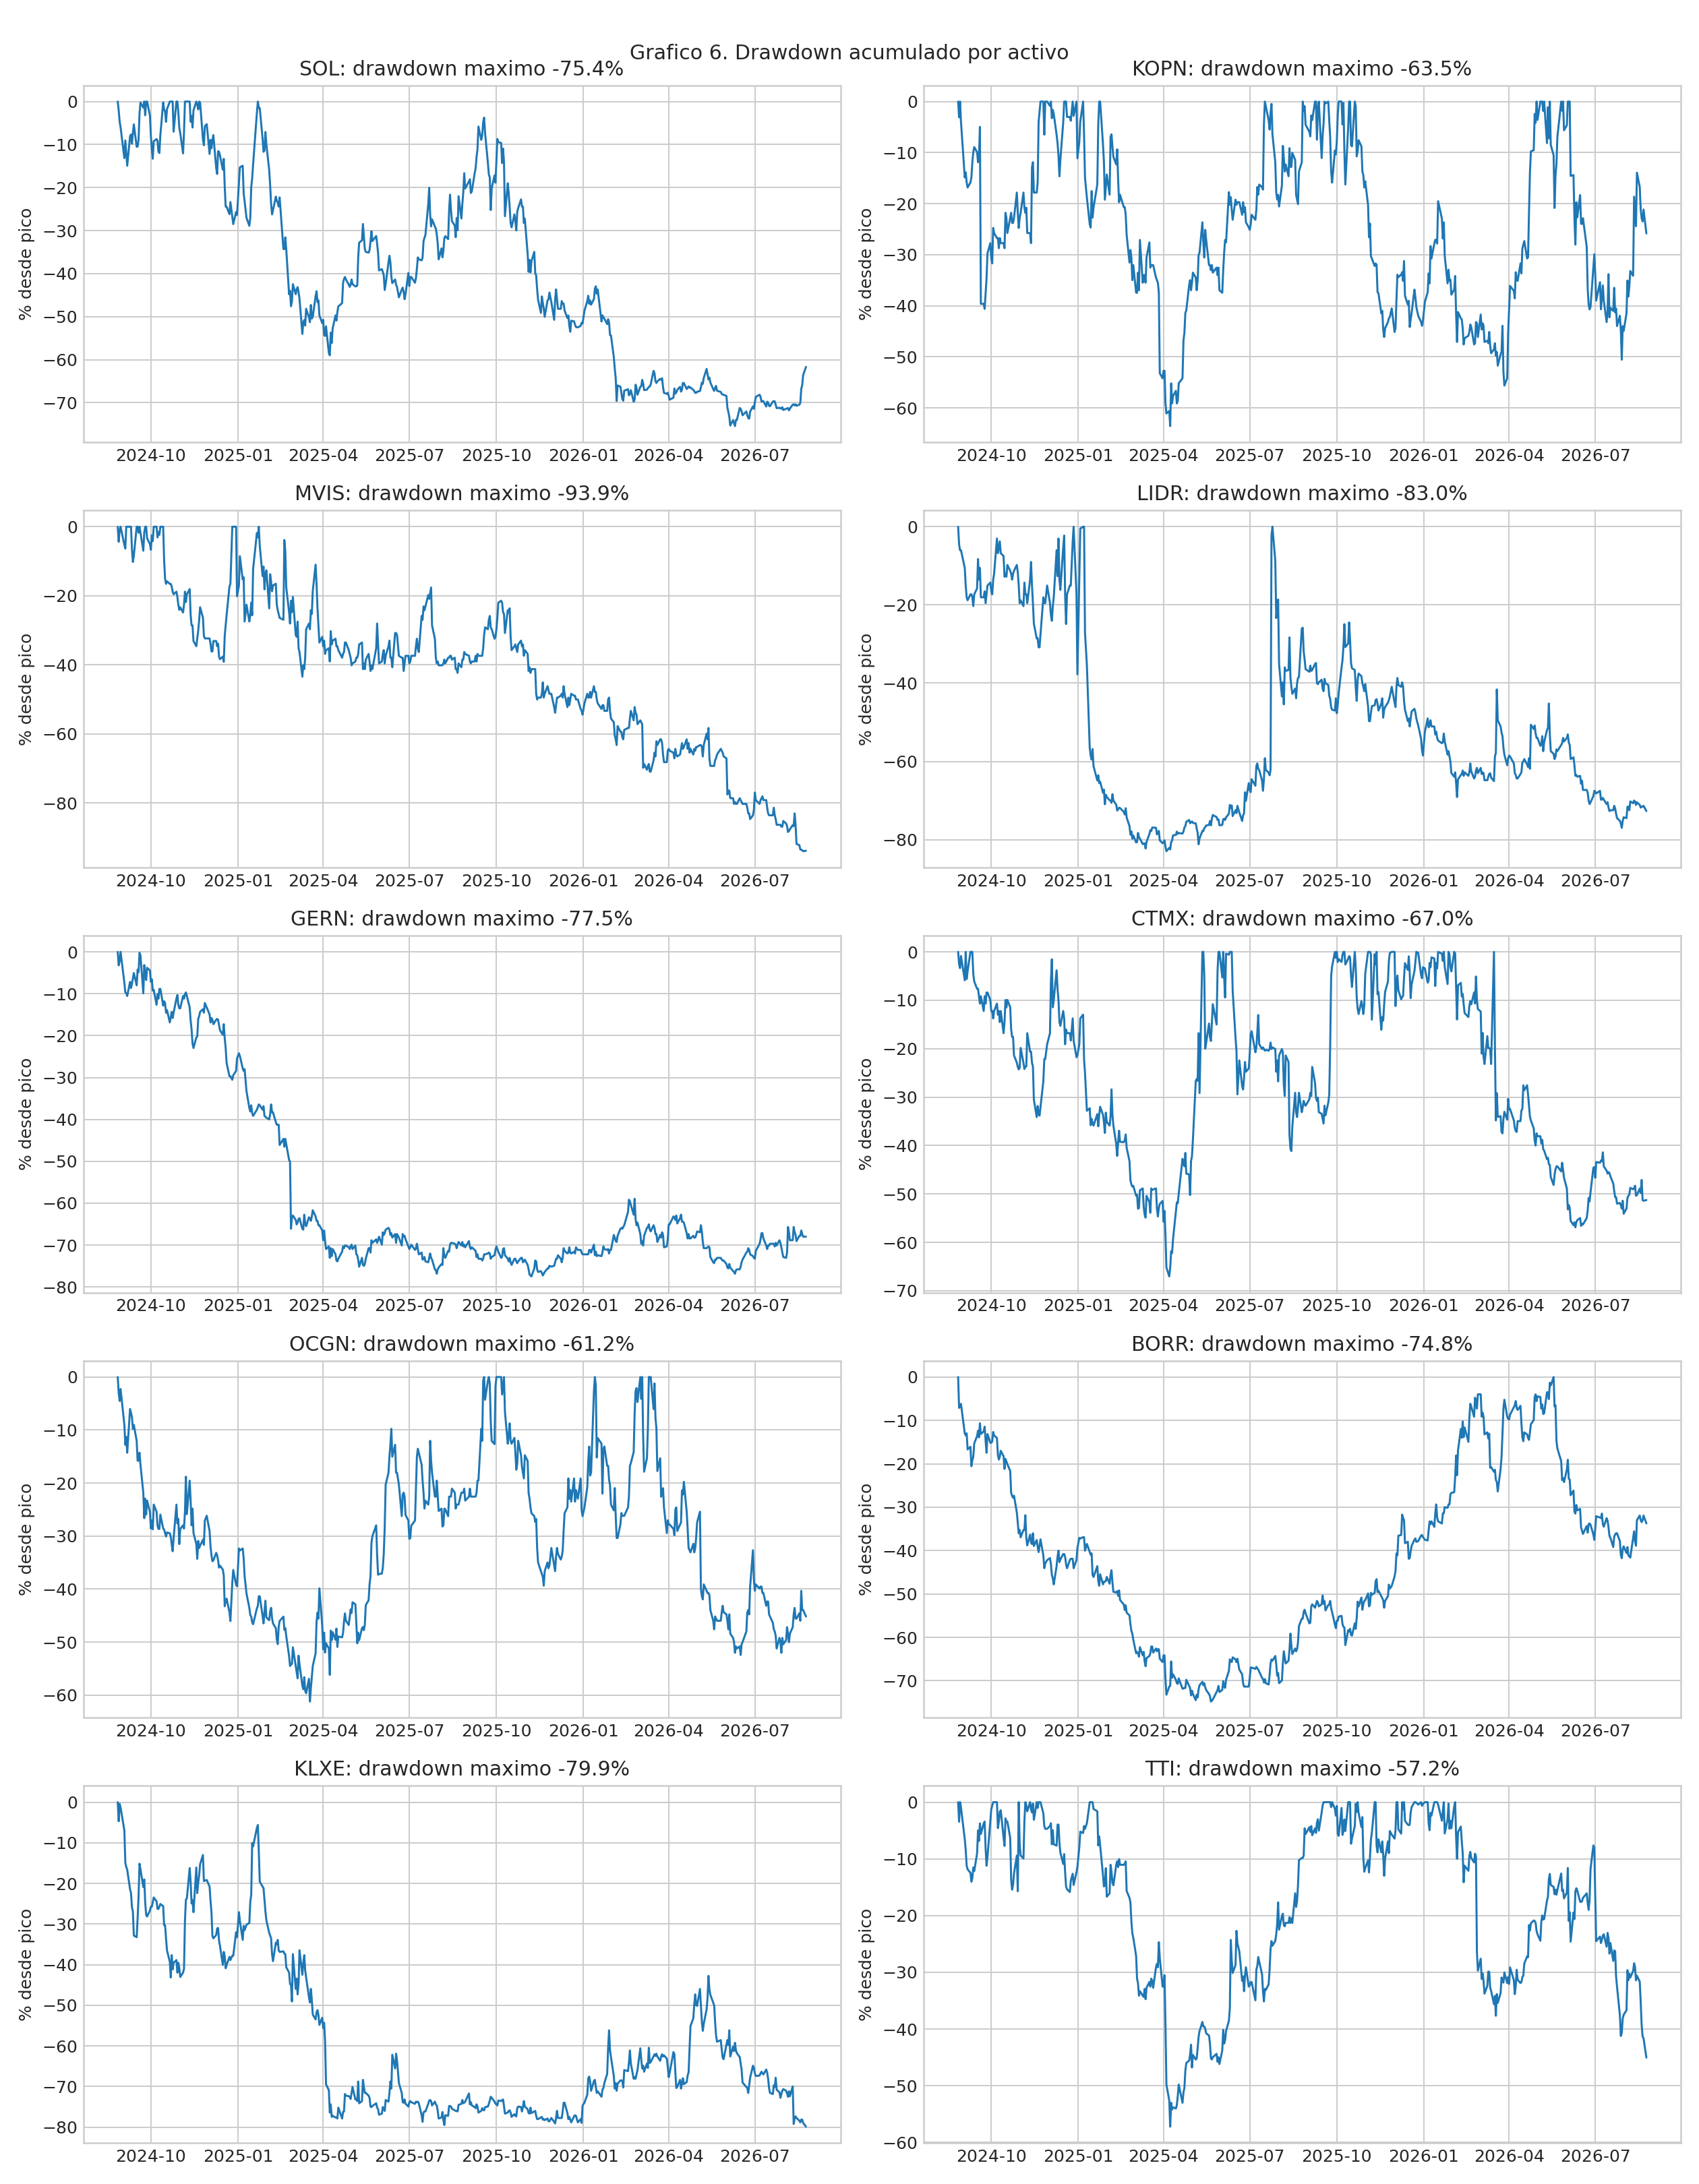
\includegraphics[width=0.82\linewidth]{grafico_6_drawdown_acumulado_todos.png}
\caption{Trayectoria de Max Drawdown acumulado. Destaca la caída de \texttt{MVIS} (-93.9\%) y la severa contracción de \texttt{SOL} (-75.45\%).}
\label{fig:drawdown}
\end{figure}

Como muestra la Tabla \ref{tab:riesgo} y la Figura \ref{fig:drawdown}, activos como \texttt{MVIS} llegaron a perder el \textbf{93.9\% de su valor}, mientras que \texttt{SOL} cayó un \textbf{75.4\%}. Adicionalmente, en acciones de bajo precio como \texttt{LIDR} y \texttt{KLXE}, la iliquidez crea una trampa peligrosa: cuando el mercado cae, no hay compradores suficientes y resulta imposible vender sin asumir pérdidas aún mayores.

\section{Respuestas a las Preguntas Clave del Estudio}

\begin{enumerate}[leftmargin=*]
    \item \textbf{¿Los activos son más sensibles que el mercado?:} Sí. Activos como \texttt{KLXE} ($\beta=1.94$) y \texttt{KOPN} ($\beta=1.82$) duplican los movimientos de sus sectores.
    \item \textbf{¿Pagan un retorno justo por su riesgo?:} No la mayoría. 6 de los 10 activos destruyen valor frente a lo exigido por CAPM.
    \item \textbf{¿Todas las acciones de bajo precio se comportan igual?:} No. Existen diferencias marcadas: mientras \texttt{TTI} logró defender el capital con un alfa moderado, \texttt{MVIS} colapsó casi por completo.
    \item \textbf{¿Qué ocurre en los peores días de mercado?:} Cuando el mercado cae, la reactividad de estos activos se dispara aún más (beta bajista superior a 2.0), acentuando las pérdidas.
\end{enumerate}

\section{Recomendación Final para Doña Victoria}

Explicado en términos sencillos y aplicables para la familia, presentamos la propuesta para cada uno de los tres mandatos de inversión:

\begin{description}[leftmargin=3.2cm]
    \item[\textbf{1. Conservación:}] \textbf{Rechazar el 100\% de estos 10 expedientes.} Ninguna de estas opciones es segura. Para no arriesgar el patrimonio a caídas del 70\% o 90\%, el dinero debe colocarse en Títulos del Tesoro (\texttt{DGS3MO}) a tasa libre de riesgo.
    \item[\textbf{2. Crecimiento:}] \textbf{Invertir en ETF de Mercado, no en acciones individuales.} Se debe evitar comprar acciones baratas individuales por su alta fragilidad. El crecimiento patrimonial debe buscarse mediante fondos indexados diversificados (\texttt{XLK}, \texttt{XLE}, \texttt{XBI}).
    \item[\textbf{3. Especulación:}] \textbf{Asignación Táctica con Presupuesto de Pérdida (1\% a 2\% máximo).} Si se desea participar en activos de alto potencial (\texttt{SOL}, \texttt{KOPN} o \texttt{TTI}), solo se debe destinar una fracción pequeña del portafolio (entre 1\% y 2\%), acompañada obligatoriamente de un límite de pérdida estricto (\textit{stop-loss} del 15\%) para cortar cualquier caída a tiempo.
\end{description}

\section{Conclusión}
El retorno del 25\% anual sin caídas es técnicamente irrealizable. El papel de la ciencia de datos en la valoración de activos no es prometer milagros insostenibles, sino medir con claridad la factura del riesgo y proteger el patrimonio familiar frente a la ruina.

\end{document}
